\documentclass[tikz,border=10pt]{standalone}
\usepackage{tikz}
\usetikzlibrary{shapes.geometric, arrows.meta, positioning, calc, fit, backgrounds}

\begin{document}
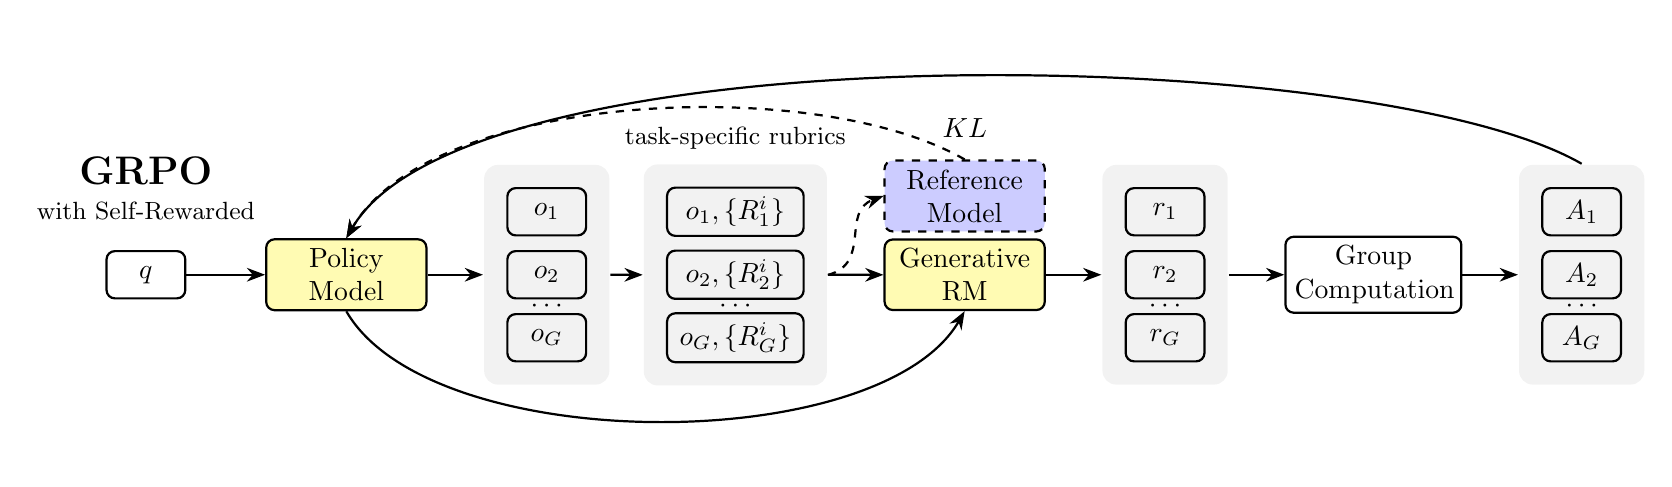
\begin{tikzpicture}[
    % Define styles
    box/.style={rectangle, draw=black, thick, minimum width=2cm, minimum height=0.8cm, rounded corners=3pt, text width=1.8cm, align=center},
    model/.style={box, fill=blue!20},
    policy/.style={box, fill=yellow!30},
    compute/.style={box, minimum width=2.2cm, text width=2cm},
    small/.style={box, minimum width=1cm, minimum height=0.6cm, text width=, align=center},
    arrow/.style={->, >=Stealth, thick},
    group_box/.style={rectangle, draw=gray!60, thick, fill=gray!10, rounded corners=5pt, inner sep=8pt},
    ]

    % Main nodes
    \node[small] (q) at (0, 0) {$q$};
    \node[font=\Large\bfseries] (title) at ($(q.north) + (0,1.0)$) {GRPO};
    \node[font=\small] (subtitle) at ($(title.south) - (0,0.2)$) {with Self-Rewarded};
    \node[policy, right=1cm of q] (policy) {Policy\\Model};

    % Output nodes from Policy Model
    \node[small, right=1cm of policy, yshift=0.8cm] (o1) {$o_1$};
    \node[small, right=1cm of policy] (o2) {$o_2$};
    \node[small, right=1cm of policy, yshift=-0.8cm] (oG) {$o_G$};
    \node at ($(o2)!0.5!(oG)$) {$\cdots$};

    % Gray box around output nodes (on background layer)
    \begin{scope}[on background layer]
        \node[group_box, draw=none, fit=(o1)(o2)(oG)] (output_group) {};
    \end{scope}

    % Output nodes with Rubrics
    \node[small, text width=1.5cm, right=1cm of o1] (o1r) {$o_1, \{R_1^{i}\}$};
    \node[small, text width=1.5cm, right=1cm of o2] (o2r) {$o_2, \{R_2^{i}\}$};
    \node[small, text width=1.5cm, right=1cm of oG] (oGr) {$o_G, \{R_G^{i}\}$};
    \node at ($(o2r)!0.5!(oGr)$) {$\cdots$};

    \begin{scope}[on background layer]
        \node[group_box, draw=none, fit=(o1r)(o2r)(oGr)] (output_rubric_group) {};
    \end{scope}

    % Label for rubrics group
    \node[above=0.05cm of output_rubric_group, font=\small] {task-specific rubrics};

    % Reference and Reward Models
    \node[model, dashed, right=1cm of o1r, yshift=0.2cm
    ] (ref) {Reference\\Model};
    \node[policy, right=1cm of o2r] (reward) {Generative\\RM};

    % Reward outputs
    \node[small, right=1cm of reward, yshift=0.8cm] (r1) {$r_1$};
    \node[small, right=1cm of reward] (r2) {$r_2$};
    \node[small, right=1cm of reward, yshift=-0.8cm] (rG) {$r_G$};
    \node at ($(r2)!0.5!(rG)$) {$\cdots$};

    % Gray box around reward outputs (on background layer)
    \begin{scope}[on background layer]
        \node[group_box, draw=none, fit=(r1)(r2)(rG)] (reward_group) {};
    \end{scope}

    % Group Computation
    \node[compute, right=1cm of r2] (group) {Group\\Computation};

    % Final outputs
    \node[small, right=1cm of group, yshift=0.8cm] (A1) {$A_1$};
    \node[small, right=1cm of group] (A2) {$A_2$};
    \node[small, right=1cm of group, yshift=-0.8cm] (AG) {$A_G$};
    \node at ($(A2)!0.5!(AG)$) {$\cdots$};

    % Gray box around final outputs (on background layer)
    \begin{scope}[on background layer]
        \node[group_box, draw=none, fit=(A1)(A2)(AG)] (final_group) {};
    \end{scope}

    % Arrows
    \draw[arrow] (q) -- (policy);
    \draw[arrow] (policy) -- (output_group);

    % Arrows from output group to models
    \draw[arrow] (output_group) -- (output_rubric_group);
    \draw[arrow] (output_rubric_group) -- (reward);
    \draw[arrow, dashed] (output_rubric_group.east) to[out=15, in=200, looseness=1.2] (ref.west);

    % Arrows from Reward Model to reward group
    \draw[arrow] (reward) -- (reward_group);

    % Arrows from reward group to Group Computation
    \draw[arrow] (reward_group) -- (group);

    % Arrows from Group Computation to final group
    \draw[arrow] (group) -- (final_group);

    % Curved feedback arrow from final group
    \draw[arrow, looseness=0.5] (final_group.north) to[out=150, in=60] (policy.north);

    % Arrow from Reference Model to Policy Model (overlapping with feedback arrow)
    \draw[arrow, looseness=0.7, dashed] (ref.north) to[out=150, in=60] (policy.north);
    \draw[arrow, looseness=0.7] (policy.south) to[out=300, in=240] (reward.south);

    % KL label between the two curved arrows
    \node at ($(ref.north) + (0,0.4)$) {$KL$};

\end{tikzpicture}
\end{document}